% cSpell: disable
\section{Inverse Problems}

\begin{frame}[plain,c]
    %\frametitle{A first slide}

    \begin{center}
        \color{DarkBlue}
    \Huge \thesection. \insertsection
    \end{center}

\end{frame}

\begin{frame}{Linear Inverse Problems}
    % introduce linear inverse problems
    % To leverage this type of redundancy, we introduce the concept of \textbf{Linear Inverse Problems}:
    % \textbf{Linear Inverse Problems}:
    \begin{equation*}
        \tikzmarknode{A}{\highlight{green}{$\Ab$}} \tikzmarknode{x}{\highlight{blue}{$\xb$}} = \tikzmarknode{y}{\highlight{yellow}{$\yb$}}
    \end{equation*}
    \vspace{2.5\baselineskip}
    \begin{tikzpicture}[overlay,remember picture,>=stealth,nodes={align=left,inner ysep=1pt},<-]
        % For "A"
        \onslide<6>{
        \path (A.south) ++ (0,-2em) node[anchor=south east,color=DarkGreen!77] (exp_A){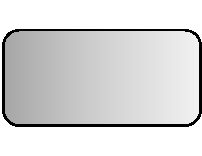
\includegraphics[width=0.05\textwidth]{Figures/intro_figures/smiley_prior_forw_op.pdf}};
        \draw [color=DarkGreen!87](A.south) |- ([xshift=-0.3ex,color=DarkGreen]exp_A.south west);
        }
        \onslide<7->{
        \path (A.south) ++ (0,-2em) node[anchor=south east,color=DarkGreen!77] (exp_A){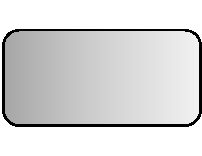
\includegraphics[width=0.05\textwidth]{Figures/intro_figures/smiley_prior_forw_op.pdf} \textbf{Measurement operator}};
        \draw [color=DarkGreen!87](A.south) |- ([xshift=-0.3ex,color=DarkGreen]exp_A.south west);
        }
        % For "x"
        \onslide<2>{
            \path (x.south) ++ (0, -4.5em) node[anchor=south east,color=blue!67] (exp_x){
\includegraphics[width=0.05\textwidth]{Figures/intro_figures/smiley_prior_x.pdf}};
        \draw [color=blue!87](x.south) |- ([xshift=-0.3ex,color=blue]exp_x.south west);
        }
        \onslide<3->{
        \path (x.south) ++ (0, -4.5em) node[anchor=south east,color=blue!67] (exp_x){
\includegraphics[width=0.05\textwidth]{Figures/intro_figures/smiley_prior_x.pdf} \textbf{Signal to reconstruct}};
        \draw [color=blue!87](x.south) |- ([xshift=-0.3ex,color=blue]exp_x.south west);
        }
        % For "y"
        \onslide<4>{
            \path (y.south) ++ (0, -1em) node[anchor=north west,color=amber!67] (exp_y){
\includegraphics[width=0.05\textwidth]{Figures/intro_figures/smiley_prior_y.pdf}};
            \draw [color=amber!87](y.south) |- ([xshift=-0.3ex,color=amber]exp_y.south east);
        }
        \onslide<5->{
        \path (y.south) ++ (0, -1em) node[anchor=north west,color=amber!67] (exp_y){
\includegraphics[width=0.05\textwidth]{Figures/intro_figures/smiley_prior_y.pdf} \textbf{Measurements}};
        \draw [color=amber!87](y.south) |- ([xshift=-0.3ex,color=amber]exp_y.south east);
        }
    \end{tikzpicture}


    \onslide<8->{
    % Problems arise when $\ker{\Ab} \neq \{0\}$, i.e. when there are multiple solutions to this equation.
    Problem: Multiple solutions!
    }

    \onslide<9->{
    \hfill \break
    % In order to select one of these solutions, we need to use a priori knowledge.
    To select one of these solutions, we need a priori knowledge.
    }
\end{frame}

\begin{frame}{Another look at redundancy}
    % give a sense of what structure is and how it relates to redundancy
    % Redundancy is not always strict: we may only have a strong correlation between 2 structures of the image.
    \only<1>{
        \begin{figure}
            \centering
            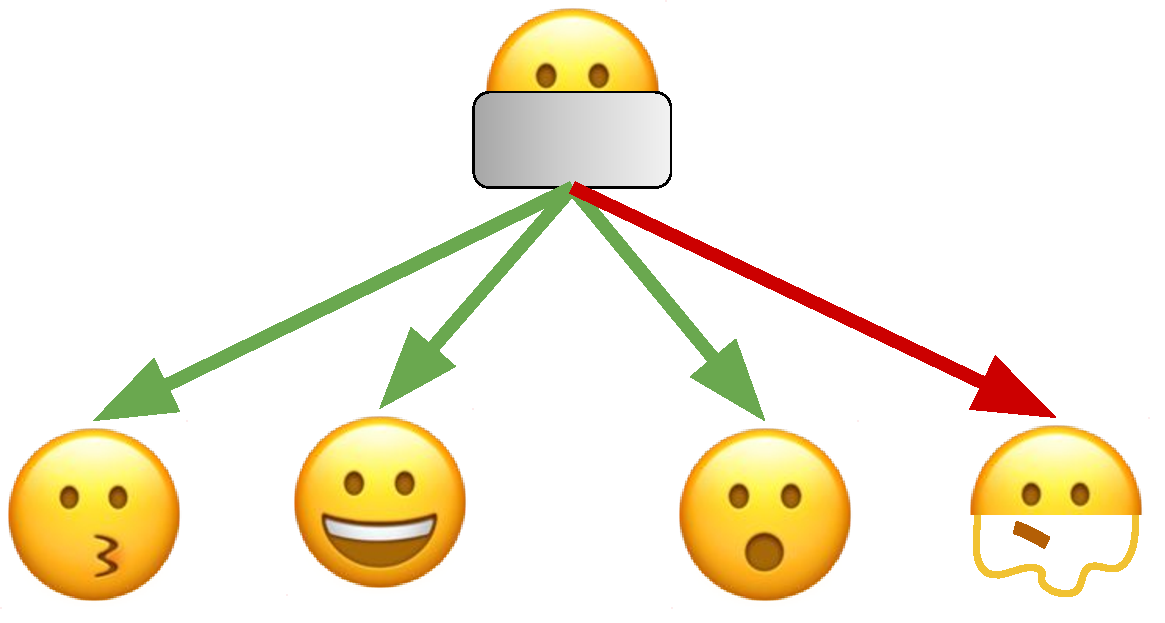
\includegraphics[height=0.5\textheight]{Figures/cs_figures/smiley_prior.pdf}
            \caption{\label{fig:redundancy-smiley}\textbf{A smiley example to a priori knowledge.}
            % Even if we do not have access to the whole image, we still know which images are more \emph{likely} to correspond to it.
            }
        \end{figure}
    }
    \only<2->{
        \begin{center}
            \begin{tikzpicture}[font=\large,>=stealth,node distance=1.5em, remember picture]
                % node
                \node(f_smiley) {$\tikzmarknode{f}{f}\left(\adjincludegraphics[valign=c,width=0.1\textwidth]{Figures/intro_figures/smiley_prior_x.pdf}\right) = $};
                \node(arrow) [right=of f_smiley.east, single arrow,bottom color=green,top color=red, minimum size=2cm,rotate=90, yshift=-1em, xshift=-1em] {};
                \node(likely_smiley) [above=0.2em of arrow.east] {Not smiley-like};
                \node(unlikely_smiley) [below=0.2em of arrow.west] {Smiley-like};
                \node(f_exp) [below=of f] {Regularizer};
                % arrow
                \draw [line width=0.1em] ($(f.south)+(0,-0.1cm)$) -- (f_exp.north);
            \end{tikzpicture}
        \end{center}
    }
\end{frame}



\begin{frame}{Application to MRI}
    % MR images themselves cannot be represented as sparse vectors directly, we need a way to express them as such.
    % MR images are not sparse as is.
    % \citet{Lustig2007} did that by using the fact that MR images can be represented sparsely in a \textbf{wavelet} basis.
    % \citet{Lustig2007} expressed their sparsity in a \textbf{wavelet} basis.

    \vspace{8ex}\break
    The Inverse Problem becomes:
    \begin{equation*}
        \hspace{3cm} \tikzmarknode{FS}{\highlight{green}{$\mathcal{F}_{\Omega}\Sbb$}} \tikzmarknode{x}{\highlight{blue}{$\xb$}} = \tikzmarknode{y}{\highlight{yellow}{$\ybb$}}
    \end{equation*}
    \begin{tikzpicture}[overlay,remember picture,>=stealth,nodes={align=left,inner ysep=1pt},<-]
        % For "FS"
        \onslide<4->{
        \path (FS.south) ++ (0,-4em) node[anchor=south east,color=DarkGreen!77,align=right, rectangle split,rectangle split horizontal, rectangle split parts=2] (exp_FS){
            \textbf{$\mathcal{F}_{\Omega}$ : per-coil FT on the $\Omega$ set;}\\
            \textbf{$\Sbb=[\Sb_1^H,\ldots, \Sb_L^H]^\top$: the sensitivity maps}\\
            \textbf{per coil}
            \nodepart{two}
            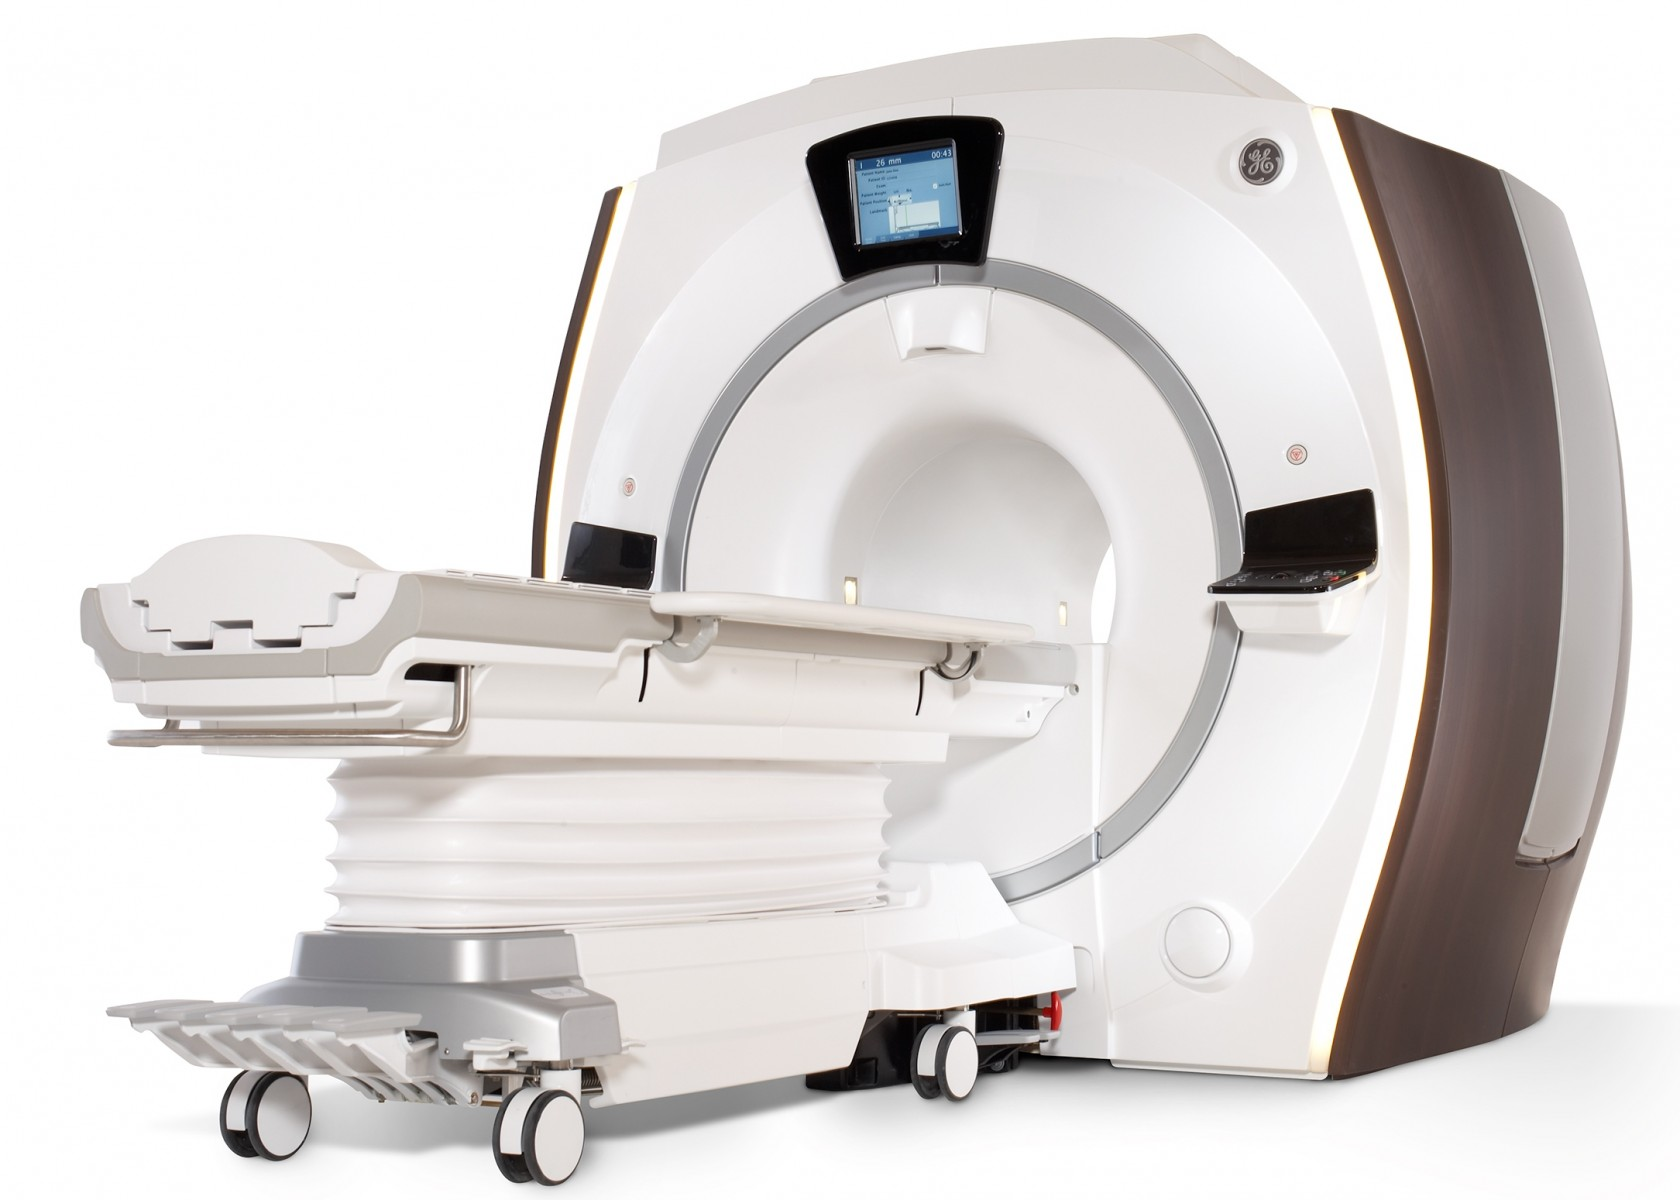
\includegraphics[width=0.08\textwidth]{Figures/intro_figures/mri.jpg}
        };
        \draw [color=DarkGreen!87](FS.south) |- ([xshift=-0.3ex,color=DarkGreen]exp_FS.south west);
        }
        % For "x"
        \onslide<2->{
        \path (x.south) ++ (0, -4em) node[anchor=south west,color=blue!67, rectangle split,rectangle split horizontal, rectangle split parts=2] (exp_x){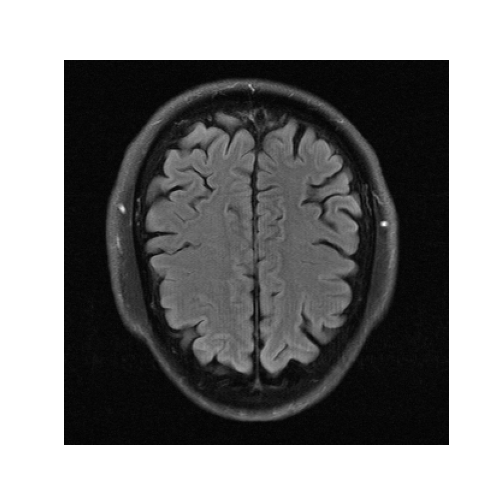
\includegraphics[trim=3.3em 3.3em 3.3em 3.3em, clip,width=0.08\textwidth,angle=180]{Figures/intro_figures/brain_mri.png} \nodepart{two} \textbf{2D or 3D MR image $\in \mathbb{C}$}};
        \draw [color=blue!87](x.south) |- ([xshift=-0.3ex,color=blue]exp_x.south east);
        }
        % For "y"
        \onslide<3->{
        \path (y.north) ++ (0, 1em) node[anchor=south west,color=amber!67, rectangle split,rectangle split horizontal, rectangle split parts=2] (exp_y){

            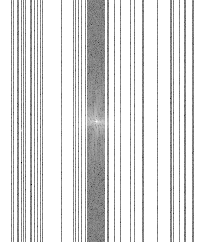
\includegraphics[width=0.06\textwidth]{Figures/intro_figures/kspace_mri.png}
            \nodepart{two} $\ybb=[\yb_1^H, \ldots, \yb_L^H]^\top$,\\ \textbf{k-space measurements} \\ \textbf{for each coil}
        };
        \draw [color=amber!87](y.north) |- ([xshift=-0.3ex,color=amber]exp_y.south east);
        }
    \end{tikzpicture}

    \onslide<4>{
        \vspace{4em}
        \begin{multicols}{2}
            \begin{center}
                $\Sbb$\\
                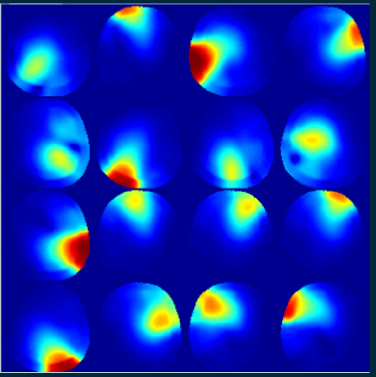
\includegraphics[height=0.2\textheight]{Figures/cs_figures/smaps.png}
            \end{center}
            \newpage
            \begin{center}
                $\Omega$
                \vspace{-3ex}
            \begin{multicols}{2}
                \begin{center}
                    Cartesian

                    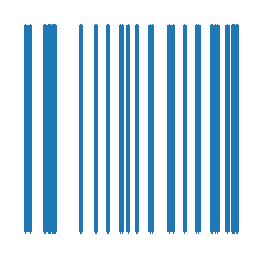
\includegraphics[height=0.2\textheight]{Figures/cs_figures/cartesian_traj.pdf}
                \end{center}

                \newpage
                \begin{center}
                    non-Cartesian

                    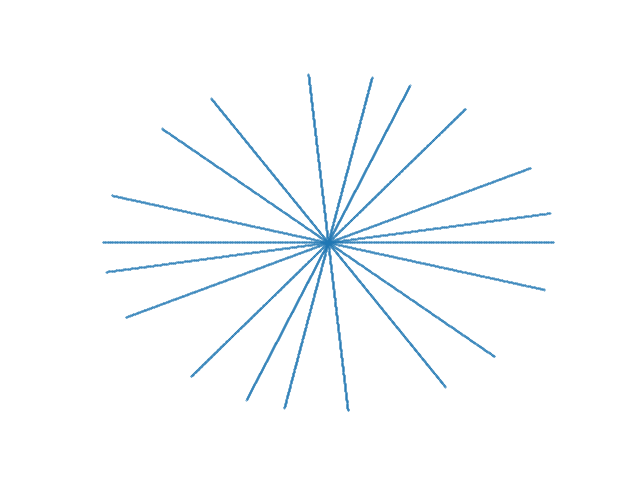
\includegraphics[height=0.2\textheight]{Figures/dl_mri_figures/radial_trajectory.png}
                \end{center}

            \end{multicols}
            \end{center}

        \end{multicols}

    }
\end{frame}

% \begin{frame}{Relaxation}
%     Can we solve the optimization problem?
%     \pause
%     No; we need to relax it using the basis pursuit:
%     \begin{equation*}
%         \label{eq:basis-pursuit}
%         \min_{\xb \in \mathbb{C}^n} \|\xb\|_1 \quad \text{subject to} \quad \Ab \xb = \yb
%     \end{equation*}

%     \pause
%     % For this problem to have the same solutions as the non-relaxed one, we need coherence-based constraints on the measurement operator $\Ab$.
%     Coherence-based constraints on $\Ab$ $\Rightarrow$ same solutions.

% \end{frame}

\begin{frame}{The canonical MRI reconstruction problem}
    % We introduce the notion of a \textbf{sparsity} basis $\psib$ (typically wavelets) and the fact that the measurements can be noisy to obtain the canonical MRI reconstruction problem:
    \begin{equation*}
        \argmin_{\xb \in \mathbb{C}^n} \overbrace{\frac12 \|\tikzmarknode{calA}{\highlight{green}{$\mathcal{A}$}} \xb - \yb \|_2^2}^{\text{\sf \footnotesize Noisy data consistency}}  + \overbrace{ \tikzmarknode{lambda}{\underline{\lambda}} \|\tikzmarknode{psi}{\highlight{brown}{$\psib$}} \xb\|_1}^{\text{\sf \footnotesize Regularization term, $\mathcal{R}$ } }
    \end{equation*}
    \vspace{\baselineskip}
    \begin{tikzpicture}[overlay,remember picture,>=stealth,nodes={align=left,inner ysep=1pt},<-]
        % For "calA"
        \path (calA.south) ++ (0,-2.5em) node[anchor=south east,color=DarkGreen!87] (exp_calA){
            $= \mathcal{F}_{\Omega}\Sbb$
        };
        \draw [color=DarkGreen!87](calA.south) |- ([xshift=-0.3ex,color=DarkGreen]exp_calA.south west);
        % For psi
        \path (psi.south) ++ (0, -2.5em) node[anchor=south west,color=brown!87] (exp_psi){
            Wavelet basis
        };
        \draw [color=brown!87](psi.south) |- ([xshift=-0.3ex,color=brown]exp_psi.south east);
        % For "lambda"
        \path (lambda.south) ++ (0, -4.5em) node[anchor=south west,color=black!87] (exp_lambda){
            Regularization hyperparameter
        };
        \draw [color=black!87](lambda.south) |- ([xshift=-0.3ex,color=black]exp_lambda.south east);
    \end{tikzpicture}
    \footnotetext{\fullcite{Lustig2007}}
\end{frame}

% \begin{frame}{ISTA}
%     %  The Iterative Shrinkage-Thresholding Algorithm~(ISTA) can be used to solve the canonical MRI reconstruction problem:
%      Iterative Shrinkage-Thresholding Algorithm~(ISTA):
%      % XXX: already highlight the steps to have a visual understanding
%      \begin{equation*}
%         \label{eq:ista-step}
%         \begin{split}
%             \xb_{n+1} &= \highlight{yellow}{$\xb_n - \epsilon_n \mathcal{A}^H\left(\mathcal{A} \xb_n - \ybb\right)$}\\
%             \xb_{n+1} &= \highlight{blue}{$\tikzmarknode{prox}{\operatorname{prox}}_{\epsilon_n \tikzmarknode{reg}{\mathcal{R}}}\left(\xb_{n+1}\right)$}
%         \end{split}
%     \end{equation*}
%     \begin{tikzpicture}[overlay,remember picture,>=stealth,nodes={align=left,inner ysep=1pt},<-]
%         % For "prox"
%         \path (prox.south) ++ (0,-2.5em) node[anchor=south east,color=black!87] (exp_prox){
%             Proximity operator
%         };
%         \draw [color=black!87](prox.south) |- ([xshift=-0.3ex,color=black]exp_prox.south west);
%         % For "reg
%         \path (reg.south) ++ (0, -2.5em) node[anchor=south west,color=black!87] (exp_reg){
%             \footnotesize $= \|\psib \cdot\|_1$
%         };
%         \draw [color=black!87](reg.south) |- ([xshift=-0.3ex,color=black]exp_reg.south east);
%     \end{tikzpicture}
% \end{frame}

% \begin{frame}{Dictionary Learning}

% \end{frame}


\begin{frame}{Limitations of classical recovery algorithms}
    % give max AF
    % also give a sense of the limitations in compute and in prior learning
    Additional acceleration factor on top of PI: 1.5.\footfullcite{knc} % from https://www.philips.fr/healthcare/ressources/landing/the-next-mr-wave/compressed-sense

    \pause
    The tool we used to express our prior knowledge, the wavelet basis, is limited: handcrafted and linear.
\end{frame}

\begin{frame}{Inverse Problems}
    \begin{block}{Recap}
        MRI is slow because of \textbf{relaxation}.

        \pause
        We can use \textbf{redundancy} in many forms to reduce the amount of samples we need in the Fourier space, and therefore the number of relaxations.

        \pause
        But we are limited by simple forms of redundancy.
    \end{block}
\end{frame}
